\documentclass[tikz,border=10pt]{standalone}
\usepackage{amsmath}
\usetikzlibrary{calc,shapes.geometric,arrows.meta,positioning}
\usepackage{xcolor}
\definecolor{accent}{HTML}{2D6BE4}
\definecolor{accentdark}{HTML}{1B4AA8}
\definecolor{codebg}{HTML}{F5F6F8}
\definecolor{failred}{HTML}{B3261E}
\newcommand{\code}[1]{\texttt{\small\detokenize{#1}}}
\begin{document}
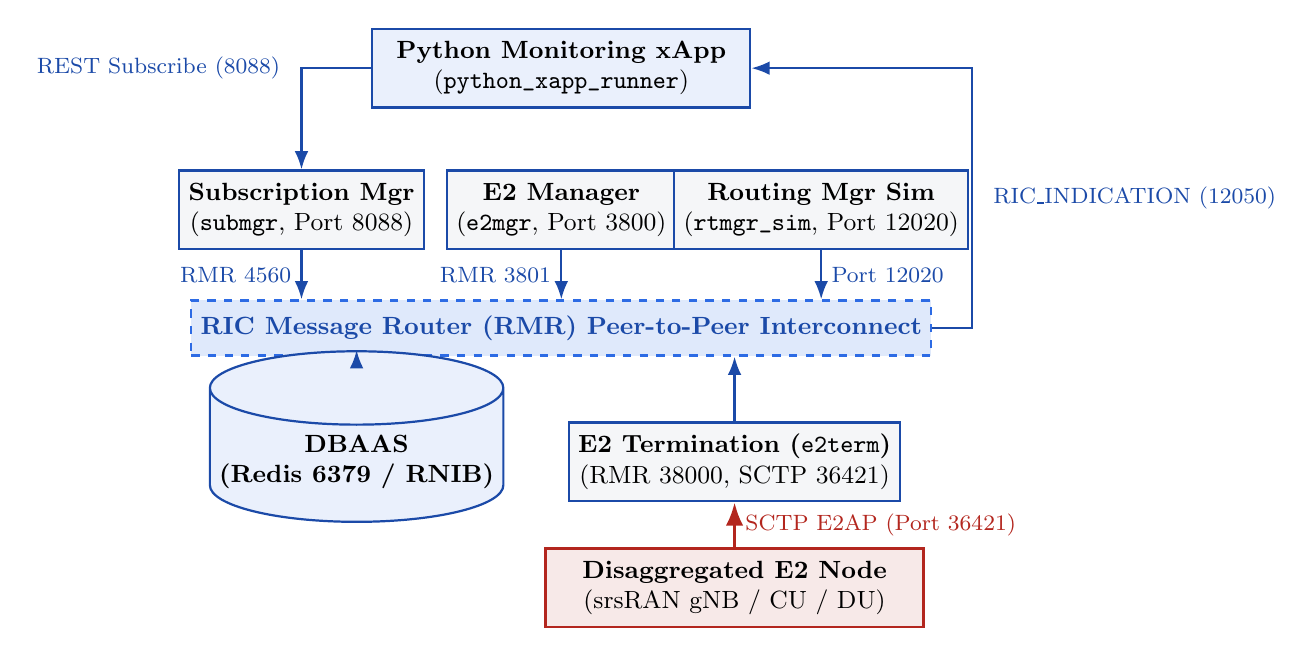
\begin{tikzpicture}[
    box/.style={rectangle, draw=accentdark, fill=codebg, thick, minimum width=2.6cm, minimum height=1.0cm, align=center, font=\small},
    db/.style={cylinder, draw=accentdark, fill=accent!10, shape border rotate=90, aspect=0.25, thick, minimum width=2.4cm, minimum height=1.1cm, align=center, font=\small\bfseries},
    rmr/.style={rectangle, draw=accent, fill=accent!15, dashed, thick, minimum width=9.2cm, minimum height=0.7cm, align=center, font=\small\bfseries\color{accentdark}},
    arrow/.style={-Latex, thick, color=accentdark},
    sctparrow/.style={-Latex, very thick, color=failred}
  ]
  % Top level: xApp
  \node[box, fill=accent!10, minimum width=4.8cm] (xapp) at (0, 3.8) {\textbf{Python Monitoring xApp}\\(\code{python_xapp_runner})};

  % Middle level: Core services
  \node[box] (submgr) at (-3.3, 2.0) {\textbf{Subscription Mgr}\\(\code{submgr}, Port 8088)};
  \node[box] (e2mgr) at (0, 2.0) {\textbf{E2 Manager}\\(\code{e2mgr}, Port 3800)};
  \node[box] (rtmgr) at (3.3, 2.0) {\textbf{Routing Mgr Sim}\\(\code{rtmgr_sim}, Port 12020)};
  
  % RMR bus
  \node[rmr] (rmrbus) at (0, 0.5) {RIC Message Router (RMR) Peer-to-Peer Interconnect};
  
  % Bottom level: Data & Termination
  \node[db] (dbaas) at (-2.6, -1.2) {\textbf{DBAAS}\\(Redis 6379 / RNIB)};
  \node[box, minimum width=3.4cm] (e2t) at (2.2, -1.2) {\textbf{E2 Termination (\code{e2term})}\\(RMR 38000, SCTP 36421)};
  
  % External: E2 Node
  \node[box, fill=failred!10, draw=failred, minimum width=4.8cm] (e2node) at (2.2, -2.8) {\textbf{Disaggregated E2 Node}\\(srsRAN gNB / CU / DU)};

  % Direct clean non-overlapping connections
  \draw[arrow] (xapp.west) -| node[midway, left=4pt, font=\footnotesize] {REST Subscribe (8088)} (submgr.north);
  \draw[arrow] (submgr.south) -- node[left, font=\footnotesize] {RMR 4560} (submgr.south |- rmrbus.north);
  \draw[arrow] (e2mgr.south) -- node[left, font=\footnotesize] {RMR 3801} (e2mgr.south |- rmrbus.north);
  \draw[arrow] (rtmgr.south) -- node[right, font=\footnotesize] {Port 12020} (rtmgr.south |- rmrbus.north);

  \draw[arrow] (rmrbus.south -| dbaas.north) -- (dbaas.north);
  \draw[arrow] (e2t.north) -- (rmrbus.south -| e2t.north);
  \draw[sctparrow] (e2node.north) -- node[right, font=\footnotesize, color=failred] {SCTP E2AP (Port 36421)} (e2t.south);
  \draw[arrow] (rmrbus.east) -- ++(0.5, 0) -- node[midway, right=4pt, font=\footnotesize] {RIC\_INDICATION (12050)} ++(0, 3.3) -- (xapp.east);
\end{tikzpicture}
\end{document}
